\chapter{Respiración celular y fermentación}\label{ch:b1:respiration-fermentation}

Un matraz de levadura en una disolución de azúcar sin aire burbujea dióxido
de carbono y convierte el azúcar en alcohol; si se deja entrar aire, el
burbujeo se frena, el alcohol cesa y la levadura crece diez veces más
deprisa con el mismo azúcar. Pasteur lo vio en 1861 y no pudo explicarlo; la
explicación costó un siglo y recorre este capítulo entero. El oxígeno
permite a una \omterm{def:b1:cell-unit-of-life:cell}{célula} extraer de la glucosa quince veces la energía que puede
obtener sin él, y lo hace pasando los electrones del azúcar por una cadena
de transportadores hasta el oxígeno, bombeando protones a través de una
membrana mientras caen y dejando después que los protones vuelvan por una
turbina que fabrica \omterm{def:b1:water-small-molecules:atp}{ATP}. Este capítulo describe la \omterm{def:b1:respiration-fermentation:glycolysis}{glucólisis}, el \omterm{def:b1:respiration-fermentation:krebs}{ciclo de
Krebs}, la \omterm{def:b1:respiration-fermentation:chain}{cadena respiratoria} y su acoplamiento quimiosmótico, las
fermentaciones que prescinden del oxígeno, y la combustión de \omterm{def:b1:lipids:triglyceride}{grasas} y
\omterm{def:b1:proteins:peptide}{proteínas} por esa misma maquinaria.

\section{La oxidación de la glucosa}

\begin{proposition}[La reacción global y sus etapas]\label{prop:b1:respiration-fermentation:overview}
\index{respiración celular}
La oxidación completa de la glucosa,
\[
\mathrm{C_6H_{12}O_6} + 6\,\mathrm{O_2} \to 6\,\mathrm{CO_2} + 6\,\mathrm{H_2O},
\qquad \Delta G^{\circ\prime} = \qty{-2870}{kJ/mol},
\]
se lleva a cabo en tres etapas que nunca dejan que los electrones se
encuentren directamente con el oxígeno. La \emph{\omterm{def:b1:respiration-fermentation:glycolysis}{glucólisis}}, en el \omterm{def:b1:eukaryotic-cell:organelle}{citosol},
escinde la glucosa en dos piruvatos y rinde 2 \omterm{def:b1:water-small-molecules:atp}{ATP} y 2 NADH. La
\emph{oxidación del piruvato y el \omterm{def:b1:respiration-fermentation:krebs}{ciclo de Krebs}}, en la \omterm{def:b1:eukaryotic-cell:mitochondrion}{matriz
mitocondrial}, oxidan el piruvato a $\mathrm{CO_2}$ y cargan los electrones
en 8 NADH y 2 $\mathrm{FADH_2}$, y fabrican 2 GTP. La \emph{fosforilación
oxidativa}, en la membrana mitocondrial interna, pasa esos electrones al
oxígeno por una cadena de transportadores que bombea protones, y el
gradiente de protones impulsa la síntesis de unos 26 \omterm{def:b1:water-small-molecules:atp}{ATP}. En total, unos 30
\omterm{def:b1:water-small-molecules:atp}{ATP} por glucosa: aproximadamente la mitad de la \omterm{prop:b1:water-small-molecules:gibbs}{energía libre} de combustión
capturada, y el resto liberado como calor.
\end{proposition}

\begin{definition}[Transportadores de electrones]\label{def:b1:respiration-fermentation:carriers}
\index{NAD}\index{FAD}
El \emph{$\mathrm{NAD^+}$} (nicotinamida adenina dinucleótido) acepta dos
electrones y un protón de un \omterm{def:b1:enzymes:enzyme}{sustrato} y se convierte en NADH; el \emph{FAD}
acepta dos electrones y dos protones y se convierte en $\mathrm{FADH_2}$.
Ambos son \omterm{def:b1:enzymes:enzyme}{coenzimas} de deshidrogenasas y ambos se reciclan: los reduce el
catabolismo y los vuelve a oxidar la \omterm{def:b1:respiration-fermentation:chain}{cadena respiratoria}. Una \omterm{def:b1:cell-unit-of-life:cell}{célula}
contiene solo micromoles de ellos, que se renuevan miles de veces por hora.
Sus potenciales redox, $E'_0 = \qty{-0.32}{V}$ para
$\mathrm{NAD^+}/\mathrm{NADH}$, los sitúan muy por debajo del oxígeno
($\qty{+0.82}{V}$): cada par de electrones que el NADH cede al oxígeno
libera $\Delta G^{\circ\prime} = -2F\Delta E =
\qty{-220}{kJ/mol}$,
suficiente para más de cuatro \omterm{def:b1:water-small-molecules:atp}{ATP}.
\end{definition}

\begin{omfigure}
\begin{tikzpicture}[font=\footnotesize, >=Stealth, line cap=round,
  st/.style={draw, thick, rounded corners=4pt, minimum height=9mm, text width=30mm, align=center, fill=white}]
  \node[st, fill=omDef!12] (gly) at (0,0) {\textbf{glucólisis}\\ citosol\\ glucosa $\to$ 2 piruvatos};
  \node[st, fill=omProp!12] (krebs) at (5.4,0) {\textbf{oxidación del piruvato}\\ \textbf{+ ciclo de Krebs}\\ matriz; 2 piruvatos $\to$ 6 $\mathrm{CO_2}$};
  \node[st, fill=omThm!12] (ox) at (10.8,0) {\textbf{fosforilación}\\ \textbf{oxidativa}\\ membrana interna; $\mathrm{O_2} \to \mathrm{H_2O}$};
  \draw[->, very thick] (gly) -- (krebs) node[midway, above, font=\scriptsize] {2 piruvatos};
  \draw[->, very thick] (krebs) -- (ox) node[midway, above, align=center, font=\scriptsize] {8 NADH\\ 2 $\mathrm{FADH_2}$};
  \draw[->, very thick] (gly.north) .. controls (0,1.8) and (10.8,1.8) .. (ox.north) node[pos=0.5, above] {2 NADH};
  \node[anchor=north, omExo!70!black] at (gly.south) {2 ATP};
  \node[anchor=north, omExo!70!black] at (krebs.south) {2 GTP};
  \node[anchor=north, omExo!70!black] at (ox.south) {$\approx$ 26 ATP};
  \node[anchor=north, align=center, gray] at (5.4,-1.75) {total $\approx$ 30 ATP por glucosa, cerca de la mitad de los \qty{2870}{kJ/mol}};
\end{tikzpicture}

{\small Las tres etapas de la respiración. La \omterm{def:b1:respiration-fermentation:glycolysis}{glucólisis} y el \omterm{def:b1:respiration-fermentation:krebs}{ciclo de Krebs}
arrancan los electrones de la glucosa y los cargan en NADH y
$\mathrm{FADH_2}$; la fosforilación oxidativa los cobra.}
\end{omfigure}

\section{La glucólisis}

\begin{definition}[Glucólisis]\label{def:b1:respiration-fermentation:glycolysis}
\index{glucólisis}
La \emph{glucólisis} es una secuencia de diez reacciones enzimáticas del
\omterm{def:b1:eukaryotic-cell:organelle}{citosol} que convierte una glucosa (C6) en dos \emph{piruvatos} (C3). En la
\emph{fase de inversión} se gastan dos \omterm{def:b1:water-small-molecules:atp}{ATP} para fosforilar el azúcar
(hexoquinasa y después \emph{fosfofructoquinasa}, PFK) y el difosfato de
seis carbonos se escinde en dos fosfatos de tres carbonos. En la \emph{fase
de beneficio} cada triosa se oxida con $\mathrm{NAD^+}$ (la única oxidación
de la glucólisis) y sus fosfatos se transfieren al ADP por
\emph{fosforilación a nivel de sustrato}\index{fosforilación a nivel de sustrato}: un fosfato cedido directamente desde un intermediario rico en
energía al ADP, sin membrana ni oxígeno. El balance:
\[
\text{glucosa} + 2\,\mathrm{NAD^+} + 2\,\mathrm{ADP} + 2\,\mathrm{P_i}
\to 2\,\text{piruvato} + 2\,\mathrm{NADH} + 2\,\mathrm{H^+} + 2\,\mathrm{ATP} + 2\,\mathrm{H_2O} .
\]
No necesita oxígeno; es la vía más antigua y más universal del
metabolismo.
\end{definition}

\begin{omfigure}
\begin{tikzpicture}[font=\footnotesize, >=Stealth, line cap=round,
  m/.style={draw, thick, rounded corners=3pt, minimum height=7mm, align=center, fill=omDef!10, inner sep=3pt},
  lab/.style={font=\scriptsize}]
  \node[m] (glc) at (0,0) {glucosa};
  \node[m] (g6p) at (3.4,0) {glucosa-6-P};
  \node[m] (f6p) at (7.0,0) {fructosa-6-P};
  \node[m] (fbp) at (10.8,0) {fructosa-1,6-bisP};
  \node[m, fill=omProp!12] (g3p) at (10.8,-2.2) {2 gliceraldehído-3-P};
  \node[m, fill=omProp!12] (bpg) at (5.6,-2.2) {2 1,3-bisfosfoglicerato};
  \node[m, fill=omProp!12] (pep) at (5.6,-4.2) {2 fosfoenolpiruvato};
  \node[m, fill=omProp!12] (pyr) at (1.0,-4.2) {2 piruvato};
  \draw[->, thick] (glc) -- (g6p) node[midway, above=3pt, omThm, font=\scriptsize] {ATP} node[midway, below=3pt, lab] {hexoquinasa};
  \draw[->, thick] (g6p) -- (f6p);
  \draw[->, thick] (f6p) -- (fbp) node[midway, above=3pt, omThm, font=\scriptsize] {ATP};
  \node[lab, anchor=north] at (8.9,-0.42) {PFK (regulada)};
  \draw[->, thick] (fbp) -- (g3p) node[midway, right, lab] {escisión en dos triosas};
  \draw[->, thick] (g3p) -- (bpg);
  \node[lab, anchor=south, omExo!70!black] at (8.6,-1.78) {2 $\mathrm{NAD^+} \to$ 2 NADH};
  \node[lab, anchor=north] at (8.6,-2.62) {oxidación};
  \draw[->, thick] (bpg) -- (pep) node[midway, right, omExo!70!black] {2 ATP};
  \draw[->, thick] (pep) -- (pyr) node[midway, above, omExo!70!black] {2 ATP};
  \node[anchor=north west, align=left, gray] at (-0.6,-5.0) {inversión: $-2$ ATP (cajas azules) \quad beneficio: $+4$ ATP, $+2$ NADH (cajas naranjas) \quad neto: $+2$ ATP, $+2$ NADH};
\end{tikzpicture}

{\small La \omterm{def:b1:respiration-fermentation:glycolysis}{glucólisis} en esquema. Se gastan dos \omterm{def:b1:water-small-molecules:atp}{ATP} para construir un
difosfato de seis carbonos, que se escinde en dos triosas; su oxidación y
dos fosforilaciones a nivel de \omterm{def:b1:enzymes:enzyme}{sustrato} devuelven en total cuatro \omterm{def:b1:water-small-molecules:atp}{ATP} y dos
NADH. La fosfofructoquinasa es la válvula de control de la vía.}
\end{omfigure}

\begin{proposition}[Control en la fosfofructoquinasa]\label{prop:b1:respiration-fermentation:pfk}
La PFK, primer paso irreversible comprometido con la \omterm{def:b1:respiration-fermentation:glycolysis}{glucólisis}, es una
\omterm{def:b1:enzymes:allosteric}{enzima alostérica} (\cref{ch:b1:enzymes}) inhibida por el \omterm{def:b1:water-small-molecules:atp}{ATP} y por el
citrato --- las señales de que la energía y el combustible del \omterm{def:b1:respiration-fermentation:krebs}{ciclo de
Krebs} abundan --- y activada por el AMP y el ADP, las señales de que no. Con
el \omterm{def:b1:water-small-molecules:atp}{ATP} alto, el flujo por la \omterm{def:b1:respiration-fermentation:glycolysis}{glucólisis} cae en segundos; cuando la \omterm{def:b1:cell-unit-of-life:cell}{célula}
gasta \omterm{def:b1:water-small-molecules:atp}{ATP}, el AMP sube bruscamente (por la adenilato quinasa,
$2\,\mathrm{ADP} \rightleftharpoons \mathrm{ATP} + \mathrm{AMP}$) y la PFK
se abre. La \emph{carga energética} de la \omterm{def:b1:cell-unit-of-life:cell}{célula} regula la vía que la
llena.
\end{proposition}

\section{Oxidación del piruvato y ciclo de Krebs}

\begin{definition}[Piruvato deshidrogenasa, acetil-CoA]\label{def:b1:respiration-fermentation:pdh}
El piruvato entra en la \omterm{def:b1:eukaryotic-cell:mitochondrion}{mitocondria} y el complejo de la \emph{piruvato
deshidrogenasa} lo oxida a \emph{acetil-CoA}\index{acetil-CoA} --- un grupo
acetilo de dos carbonos transportado por la \omterm{def:b1:enzymes:enzyme}{coenzima} A
(\cref{ch:b1:nucleic-acids}) en un enlace tioéster rico en energía ---, con
liberación de un $\mathrm{CO_2}$ y un NADH. El acetil-CoA es la entrada
común de todos los combustibles al ciclo: los \omterm{def:b1:carbohydrates:monosaccharide}{glúcidos} por el piruvato, las
\omterm{def:b1:lipids:triglyceride}{grasas} por la $\beta$-oxidación y muchos \omterm{def:b1:proteins:aminoacid}{aminoácidos} directamente.
\end{definition}

\begin{definition}[El ciclo de Krebs]\label{def:b1:respiration-fermentation:krebs}
\index{ciclo de Krebs}\index{ciclo del ácido cítrico}
El \emph{ciclo de Krebs} (ciclo del ácido cítrico), en la \omterm{def:b1:eukaryotic-cell:mitochondrion}{matriz
mitocondrial}, condensa el \omterm{def:b1:respiration-fermentation:pdh}{acetil-CoA} (C2) con el oxalacetato (C4) para dar
citrato (C6) y, en ocho pasos, oxida los dos carbonos a $\mathrm{CO_2}$
mientras regenera el oxalacetato. Por grupo acetilo: 3 NADH, 1
$\mathrm{FADH_2}$, 1 GTP (por \omterm{def:b1:respiration-fermentation:glycolysis}{fosforilación a nivel de sustrato}) y 2
$\mathrm{CO_2}$. Por glucosa (dos acetilos): 6 NADH, 2 $\mathrm{FADH_2}$, 2
GTP y 4 $\mathrm{CO_2}$, que con los 2 $\mathrm{CO_2}$ de la piruvato
deshidrogenasa dan los seis de la ecuación global. En el ciclo mismo no se
consume oxígeno; funciona solo mientras la \omterm{def:b1:respiration-fermentation:chain}{cadena respiratoria} vuelve a
oxidar su NADH. Es además \emph{anfibólico}: sus intermediarios se extraen
para la biosíntesis (\cref{ch:b1:biosyntheses-integration}) y se reponen a
partir de \omterm{def:b1:proteins:aminoacid}{aminoácidos} y de piruvato.
\end{definition}

\begin{omfigure}
\begin{tikzpicture}[font=\footnotesize, >=Stealth, line cap=round]
  \def\R{2.6}
  \foreach \a/\n/\c in {90/citrato (C6)/omDef, 45/isocitrato (C6)/omDef, 0/$\alpha$-cetoglutarato (C5)/omDef, -45/succinil-CoA (C4)/omDef, -90/succinato (C4)/omDef, -135/fumarato (C4)/omDef, 180/malato (C4)/omDef, 135/oxalacetato (C4)/omProp} {
    \node[draw, thick, rounded corners=3pt, fill=\c!12, inner sep=2.5pt, font=\scriptsize] (n\a) at (\a:\R) {\n};
  }
  \foreach \a/\b in {90/45, 45/0, 0/-45, -45/-90, -90/-135, -135/180, 180/135, 135/90} {
    \draw[->, thick] (n\a) to[bend right=25] (n\b);
  }
  % outputs
  \node[omExo!70!black, anchor=west, align=left] at (3.5,1.9) {NADH, $\mathrm{CO_2}$};
  \node[omExo!70!black, anchor=west, align=left] at (3.5,-1.6) {NADH, $\mathrm{CO_2}$};
  \node[omExo!70!black, anchor=north, align=center] at (0,-3.3) {GTP};
  \node[omExo!70!black, anchor=east, align=right] at (-3.4,-1.7) {$\mathrm{FADH_2}$};
  \node[omExo!70!black, anchor=east, align=right] at (-3.4,1.7) {NADH};
  % input
  \node[draw, thick, rounded corners=3pt, fill=omThm!15, inner sep=2.5pt, font=\scriptsize] (ac) at (0,4.3) {acetil-CoA (C2)};
  \draw[->, thick, omThm] (ac) -- (n90);
  \node[anchor=west, align=left, gray] at (3.3,4.0) {por vuelta: 3 NADH, 1 $\mathrm{FADH_2}$,\\ 1 GTP, 2 $\mathrm{CO_2}$};
\end{tikzpicture}

{\small El \omterm{def:b1:respiration-fermentation:krebs}{ciclo de Krebs}. Un grupo acetilo entra condensándose con el
oxalacetato; dos carbonos salen como $\mathrm{CO_2}$ en las dos
descarboxilaciones; las cuatro oxidaciones cargan tres NADH y un
$\mathrm{FADH_2}$; y el oxalacetato se regenera para la vuelta siguiente.}
\end{omfigure}

\begin{example}[Seguir los carbonos]\label{ex:b1:respiration-fermentation:carbons}
Dese a una \omterm{def:b1:cell-unit-of-life:cell}{célula} glucosa marcada con $\mathrm{^{14}C}$ en el carbono 1: la
marca aparece en el carbono metilo del piruvato, después en el del
\omterm{def:b1:respiration-fermentation:pdh}{acetil-CoA}, entra en el citrato y sale como $\mathrm{CO_2}$ solo en la
segunda o la tercera vuelta del ciclo, pues los dos carbonos liberados en
una vuelta dada pertenecen al oxalacetato de la anterior. Krebs (1937)
dedujo el ciclo de la observación de que cantidades catalíticas de
cualquiera de sus ácidos estimulaban la oxidación de mucho más piruvato del
que ellos mismos podían justificar: se estaban regenerando.
\end{example}

\begin{omfigure}
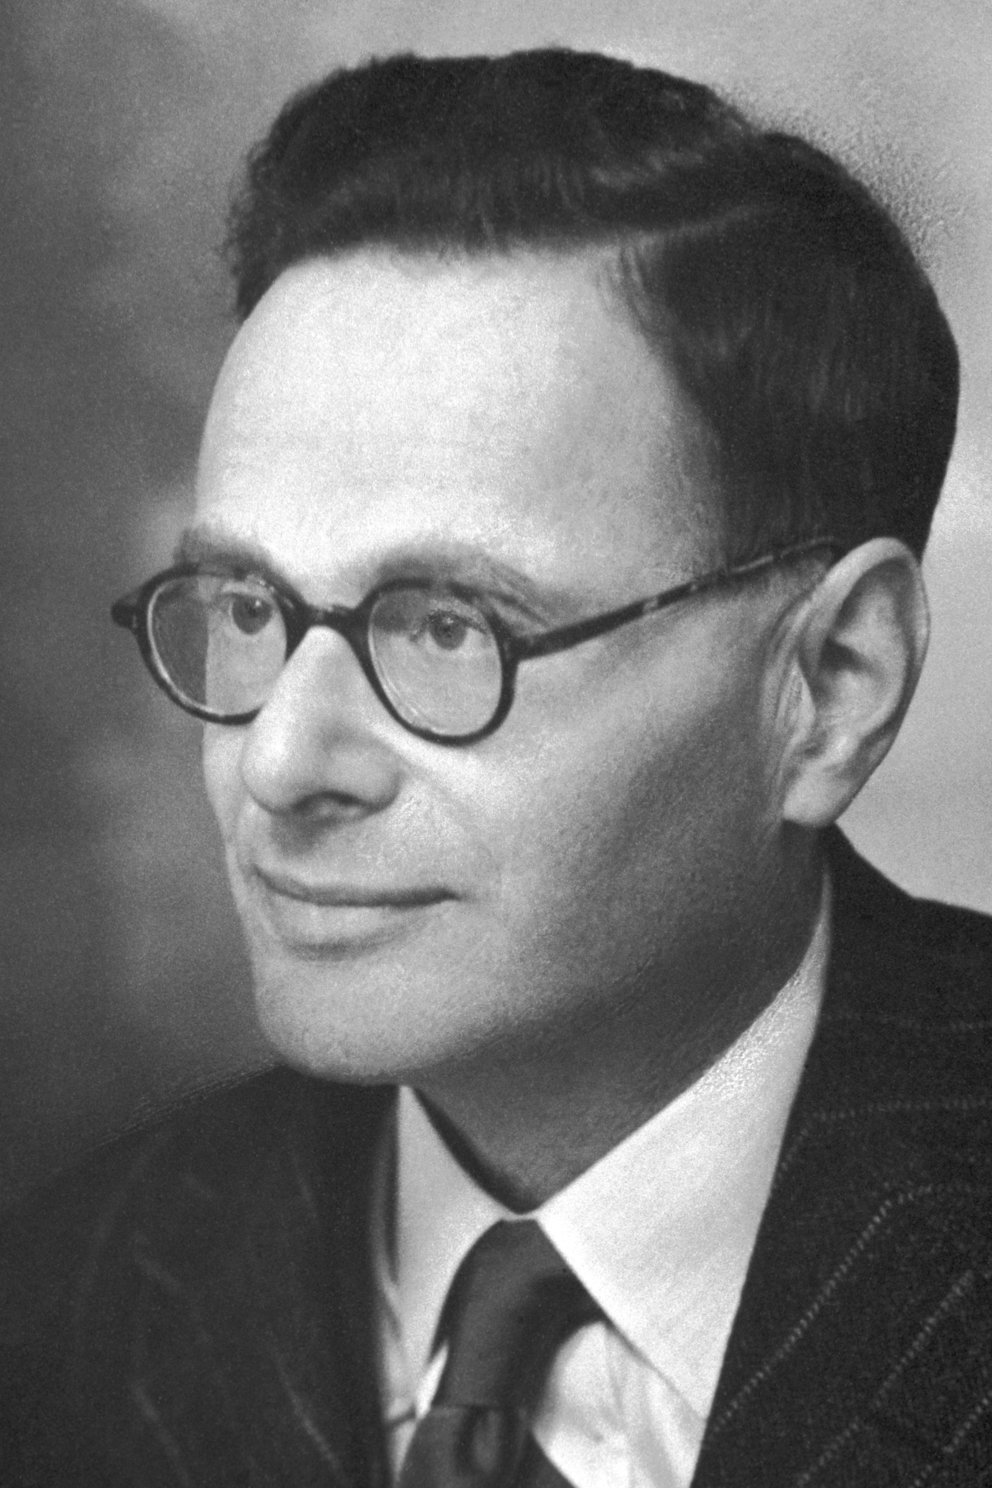
\includegraphics[width=0.26\linewidth]{images/book3/krebs.jpg}

{\small Hans Krebs (1900--1981), que dedujo el ciclo en 1937 a partir de las
velocidades con que el músculo de paloma triturado oxidaba sus ácidos.
Fotografía: Fundación Nobel, dominio público.}
\end{omfigure}

\section{La fosforilación oxidativa}

\begin{definition}[La cadena respiratoria]\label{def:b1:respiration-fermentation:chain}
\index{cadena respiratoria}\index{cadena de transporte de electrones}
La \emph{cadena respiratoria} son cuatro complejos proteicos de la membrana
mitocondrial interna y dos transportadores móviles. El NADH cede sus
electrones al \emph{complejo I}, el $\mathrm{FADH_2}$ (a través de la
succinato deshidrogenasa, el \emph{complejo II}) cede los suyos; ambos
reducen la \emph{ubiquinona} (Q), una quinona liposoluble que difunde por la
membrana; Q los pasa al \emph{complejo III}, que los entrega al
\emph{citocromo $c$}, una \omterm{def:b1:proteins:peptide}{proteína} pequeña de la cara externa; y el
\emph{complejo IV} (la citocromo oxidasa) los entrega, de cuatro en cuatro,
al $\mathrm{O_2}$, con lo que forma agua. En cada uno de los complejos I,
III y IV los electrones caen de potencial y la energía bombea protones desde
la matriz al espacio intermembranoso: unos 4, 4 y 2 por par de electrones,
diez por NADH y seis por $\mathrm{FADH_2}$ (que entra por debajo del
complejo I).
\end{definition}

\begin{omfigure}
\begin{tikzpicture}[font=\footnotesize, >=Stealth, line cap=round]
  % membrane band
  \fill[omDef!15] (0,0) rectangle (13.0,1.4);
  \draw[omDef!60!black] (0,0) -- (13.0,0) (0,1.4) -- (13.0,1.4);
  \node[anchor=east, gray, align=right] at (-0.15,1.25) {espacio\\ intermembranoso\\ (mucho $\mathrm{H^+}$, pH 7)};
  \node[anchor=east, gray, align=right] at (-0.15,0.15) {matriz\\ (poco $\mathrm{H^+}$, pH 8)};
  % complexes
  \node[draw, thick, fill=omThm!25, rounded corners=3pt, minimum height=18mm, minimum width=13mm, align=center] (c1) at (1.5,0.7) {I};
  \node[draw, thick, fill=omThm!25, rounded corners=3pt, minimum height=12mm, minimum width=10mm, align=center] (c2) at (3.6,0.5) {II};
  \node[draw, thick, fill=omThm!25, rounded corners=3pt, minimum height=18mm, minimum width=13mm, align=center] (c3) at (6.2,0.7) {III};
  \node[draw, thick, fill=omThm!25, rounded corners=3pt, minimum height=18mm, minimum width=13mm, align=center] (c4) at (8.9,0.7) {IV};
  \node[draw, thick, fill=omExo!25, rounded corners=6pt, minimum height=16mm, minimum width=12mm, align=center] (atp) at (11.6,0.5) {ATP\\ sintasa};
  \node[circle, draw, thick, fill=omProp!30, inner sep=1.5pt, font=\scriptsize] (q) at (4.9,0.55) {Q};
  \node[circle, draw, thick, fill=omProp!30, inner sep=1.5pt, font=\scriptsize] (cyt) at (7.55,1.25) {cit $c$};
  % electron flow
  \draw[->, thick, omProp] (c1) -- (q); \draw[->, thick, omProp] (c2) -- (q); \draw[->, thick, omProp] (q) -- (c3); \draw[->, thick, omProp] (c3) -- (cyt); \draw[->, thick, omProp] (cyt) -- (c4);
  % inputs
  \node[anchor=north, align=center] at (1.5,-0.5) {NADH $\to$ $\mathrm{NAD^+}$};
  \node[anchor=north, align=center] at (3.6,-0.5) {$\mathrm{FADH_2}$\\ (succinato)};
  \node[anchor=north, align=center, font=\scriptsize] at (8.6,-0.5) {$\tfrac12\,\mathrm{O_2} + 2\,\mathrm{H^+} \to \mathrm{H_2O}$};
  % proton pumping arrows
  \foreach \x/\n in {1.5/4 $\mathrm{H^+}$, 6.2/4 $\mathrm{H^+}$, 8.9/2 $\mathrm{H^+}$} {
    \draw[->, very thick, omExo!80!black] (\x+0.5,-0.05) -- (\x+0.5,1.9) node[above, font=\scriptsize] {\n};
  }
  \draw[->, very thick, omExo!80!black] (11.6,2.1) -- (11.6,1.35);
  \draw[->, very thick, omExo!80!black] (11.6,-0.35) -- (11.6,-0.75);
  \node[anchor=south, font=\scriptsize] at (11.6,2.15) {$\approx 4\,\mathrm{H^+}$ por ATP};
  \node[anchor=north, align=center, font=\scriptsize] at (11.6,-0.8) {ADP $+ \mathrm{P_i} \to$ ATP};
\end{tikzpicture}

{\small La membrana mitocondrial interna. Los electrones (naranja) caen
desde el NADH o el $\mathrm{FADH_2}$ por los complejos hasta el oxígeno; los
complejos I, III y IV bombean protones hacia fuera (verde); la \omterm{thm:b1:photosynthesis:chemiosmosis}{ATP sintasa}
los deja volver y fabrica \omterm{def:b1:water-small-molecules:atp}{ATP}.}
\end{omfigure}

\begin{theorem}[Acoplamiento quimiosmótico]\label{thm:b1:respiration-fermentation:chemiosmosis}
\index{teoría quimiosmótica}\index{fuerza protón-motriz}
El gradiente de protones construido por la cadena --- unos \qty{0.16}{V} de
\omterm{def:b1:membranes-transport:potential}{potencial de membrana} (matriz negativa) más una unidad de pH, una
\emph{\omterm{thm:b1:respiration-fermentation:chemiosmosis}{fuerza protón-motriz}} de unos \qty{0.22}{V}, o \qty{21}{kJ} por mol de
protones --- es el único vínculo entre el transporte de electrones y la
síntesis de \omterm{def:b1:water-small-molecules:atp}{ATP}. La \omterm{thm:b1:photosynthesis:chemiosmosis}{ATP sintasa}, un motor rotatorio de la membrana interna,
deja pasar unos \qty{3}{H^+} por cada \omterm{def:b1:water-small-molecules:atp}{ATP} fabricado, y se gasta uno más en
importar el fosfato y exportar el \omterm{def:b1:water-small-molecules:atp}{ATP}: 4 por \omterm{def:b1:water-small-molecules:atp}{ATP}. De ahí la \emph{relación
P/O}\index{relación P/O}: $10/4 = 2.5$ \omterm{def:b1:water-small-molecules:atp}{ATP} por NADH y $6/4 = 1.5$ por
$\mathrm{FADH_2}$.
\end{theorem}
\begin{proof}[Evidencia]
Las \omterm{def:b1:eukaryotic-cell:mitochondrion}{mitocondrias} solo fabrican \omterm{def:b1:water-small-molecules:atp}{ATP} cuando su membrana interna está intacta y
cerrada; los fragmentos que transportan electrones pero no pueden mantener
un gradiente no fabrican ninguno. Los desacoplantes, como el dinitrofenol,
que llevan protones a través de la membrana, suprimen la síntesis de \omterm{def:b1:water-small-molecules:atp}{ATP}
mientras el consumo de oxígeno continúa e incluso se acelera, y la energía
se va como calor --- la \omterm{def:b1:lipids:triglyceride}{grasa} parda lo hace a propósito con su propia
\omterm{def:b1:proteins:peptide}{proteína} desacoplante (\cref{ch:b1:mammal-organization}), y el dinitrofenol
llegó a venderse como adelgazante y mataba por hipertermia. Los \omterm{def:b1:enzymes:inhibitors}{inhibidores}
de la cadena (el cianuro sobre el complejo IV) detienen ambas cosas; los
\omterm{def:b1:enzymes:inhibitors}{inhibidores} de la sintasa (la oligomicina) detienen la síntesis de \omterm{def:b1:water-small-molecules:atp}{ATP} y,
como el gradiente no puede descargarse, detienen también la respiración, que
un desacoplante restablece. Un gradiente de pH artificial impuesto a
\omterm{def:b1:eukaryotic-cell:mitochondrion}{mitocondrias} en la oscuridad impulsa la síntesis de \omterm{def:b1:water-small-molecules:atp}{ATP}, igual que en los
\omterm{def:b1:eukaryotic-cell:plastid}{cloroplastos} (\cref{ch:b1:photosynthesis}).
\end{proof}

\begin{omfigure}
\begin{tikzpicture}
  \node[anchor=south west, inner sep=0] (img) at (0,0)
    {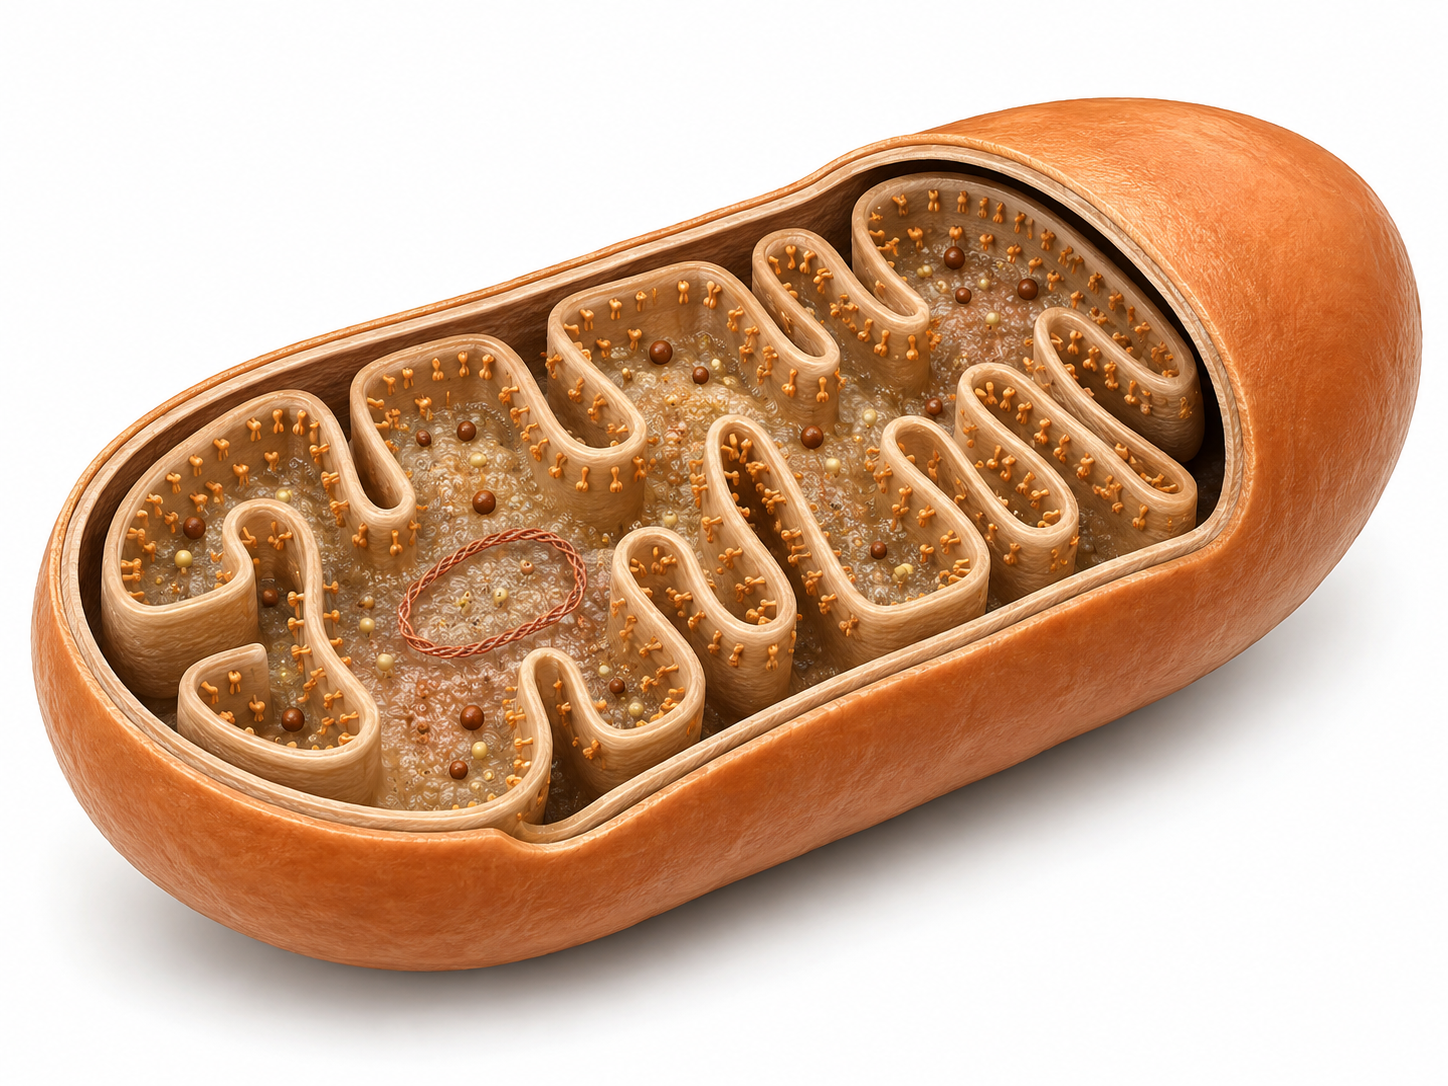
\includegraphics[width=0.50\linewidth]{images/book3/ai/fig-mitochondrion-cutaway.png}};
  \begin{scope}[x={(img.south east)}, y={(img.north west)},
      every node/.style={font=\small}]
    \draw[omDef, thick] (0.10,0.55) -- (-0.03,0.70) node[left] {membrana externa};
    \draw[omDef, thick] (0.45,0.72) -- (0.45,1.08) node[above, align=center] {membrana interna plegada en crestas:\\ la cadena respiratoria y la ATP sintasa};
    \draw[omDef, thick] (0.55,0.35) -- (1.03,0.24) node[right, align=left] {matriz: ciclo\\ de Krebs, ADN,\\ ribosomas};
    \draw[omDef, thick] (0.16,0.40) -- (-0.03,0.26) node[left] {espacio intermembranoso};
  \end{scope}
\end{tikzpicture}

{\small Una \omterm{def:b1:eukaryotic-cell:mitochondrion}{mitocondria} abierta. Los pliegues de la membrana interna
multiplican el área disponible para la cadena y la sintasa; la matriz que
encierran aloja el \omterm{def:b1:respiration-fermentation:krebs}{ciclo de Krebs}.}
\end{omfigure}

\begin{method}[El balance de ATP de una glucosa]\label{met:b1:respiration-fermentation:balance}
\begin{enumerate}
  \item \omterm{def:b1:respiration-fermentation:glycolysis}{Glucólisis}: $+2$ \omterm{def:b1:water-small-molecules:atp}{ATP} (netos), $+2$ NADH en el \omterm{def:b1:eukaryotic-cell:organelle}{citosol}.
  \item Piruvato deshidrogenasa: $+2$ NADH. \omterm{def:b1:respiration-fermentation:krebs}{Ciclo de Krebs}: $+6$ NADH, $+2$
        $\mathrm{FADH_2}$, $+2$ GTP ($=$ \omterm{def:b1:water-small-molecules:atp}{ATP}).
  \item Fosforilación oxidativa: $2.5$ \omterm{def:b1:water-small-molecules:atp}{ATP} por cada NADH mitocondrial
        (8: 20 \omterm{def:b1:water-small-molecules:atp}{ATP}) y $1.5$ por $\mathrm{FADH_2}$ (2: 3 \omterm{def:b1:water-small-molecules:atp}{ATP}).
  \item El NADH citosólico no puede atravesar la membrana interna; sus
        electrones entran por una lanzadera que los entrega al
        $\mathrm{FAD}$ (1,5 cada uno, en músculo y encéfalo) o al
        $\mathrm{NAD^+}$ (2,5 cada uno, en hígado y corazón): 3 o 5 \omterm{def:b1:water-small-molecules:atp}{ATP}.
  \item Total: $2 + 2 + 20 + 3 + 3 = 30$, o $32$ con la mejor lanzadera.
        Rendimiento: $30\times 50/2870 \approx \qty{52}{\%}$ en condiciones
        celulares.
\end{enumerate}
\end{method}

\section{La fermentación}

\begin{definition}[Fermentación]\label{def:b1:respiration-fermentation:fermentation}
\index{fermentación}
Sin oxígeno la \omterm{def:b1:respiration-fermentation:chain}{cadena respiratoria} se detiene, el NADH no puede volver a
oxidarse y la \omterm{def:b1:respiration-fermentation:glycolysis}{glucólisis} se pararía en segundos por falta de
$\mathrm{NAD^+}$. La \emph{fermentación} lo regenera usando el propio
piruvato como aceptor de electrones: en la \emph{fermentación láctica}
(músculo, glóbulos rojos, bacterias lácticas) el piruvato se reduce a
lactato; en la \emph{fermentación alcohólica} (levaduras, algunas plantas)
se descarboxila a acetaldehído, que se reduce a etanol y libera
$\mathrm{CO_2}$. El rendimiento es el de la propia \omterm{def:b1:respiration-fermentation:glycolysis}{glucólisis}: 2 \omterm{def:b1:water-small-molecules:atp}{ATP} por
glucosa, la quinceava parte del de la respiración; el carbono apenas se
oxida y los productos conservan casi toda la energía del combustible. La
\emph{respiración anaerobia} --- una \omterm{def:b1:respiration-fermentation:chain}{cadena de transporte de electrones} que
termina en nitrato, sulfato o carbonato en vez de en oxígeno, en muchas
bacterias --- es otra cosa, y se trata en el volumen del segundo año.
\end{definition}

\begin{omfigure}
\begin{minipage}[b]{0.44\linewidth}\centering
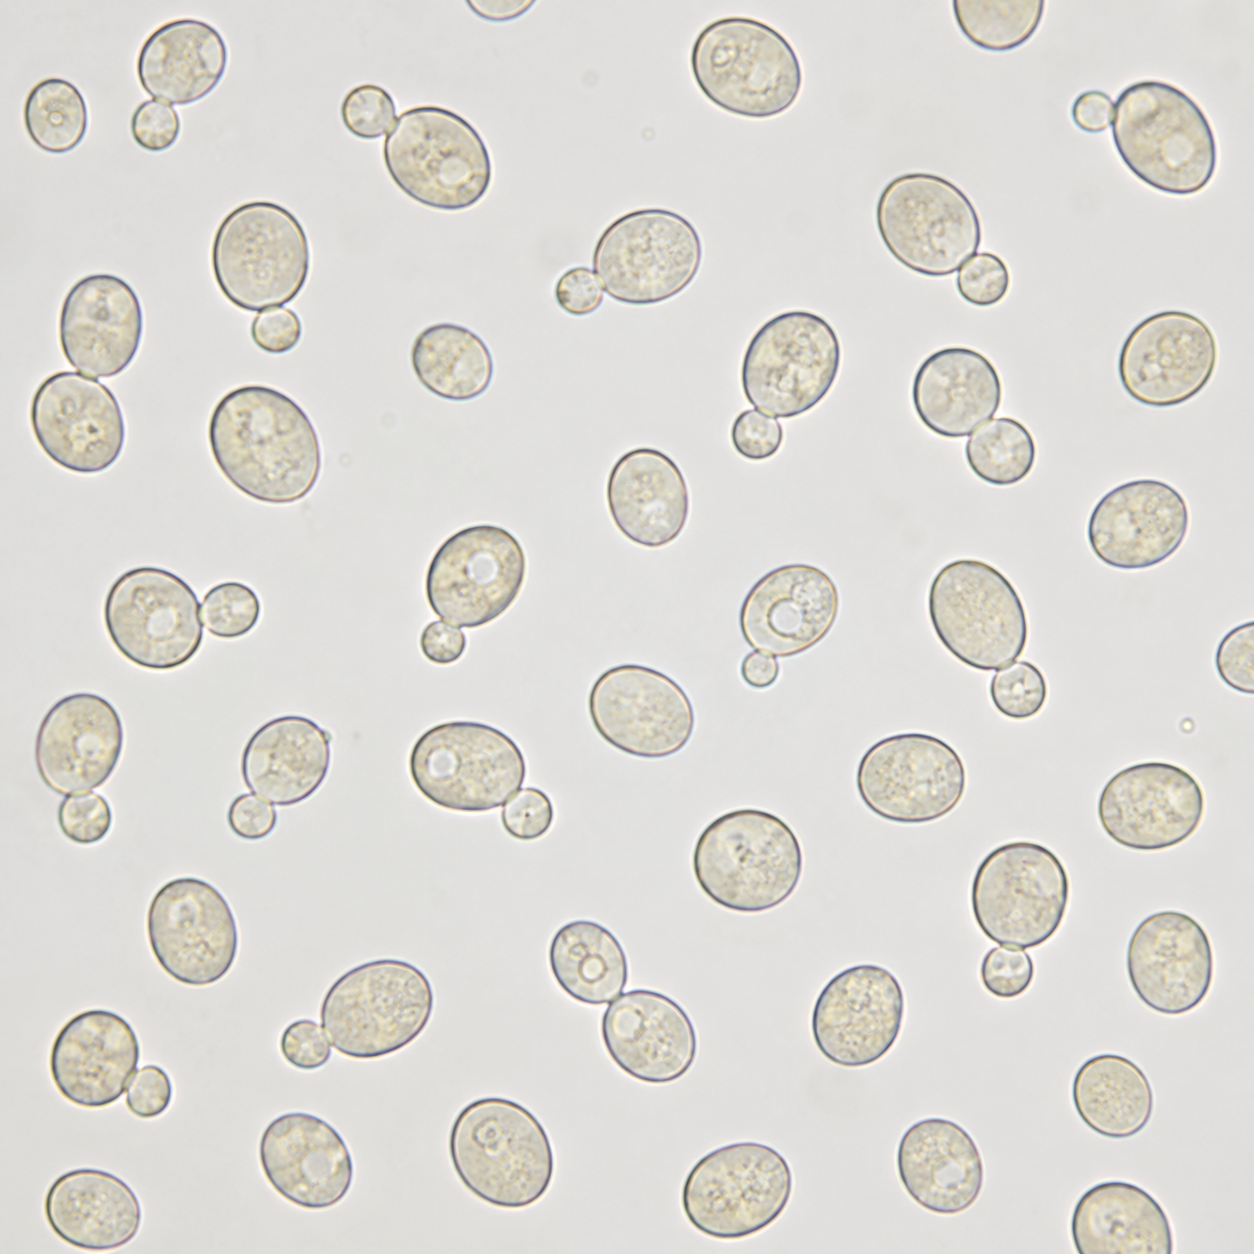
\includegraphics[width=0.9\linewidth]{images/book3/ai/b3-15-yeast-budding.png}
\end{minipage}\hfill
\begin{minipage}[b]{0.52\linewidth}\centering
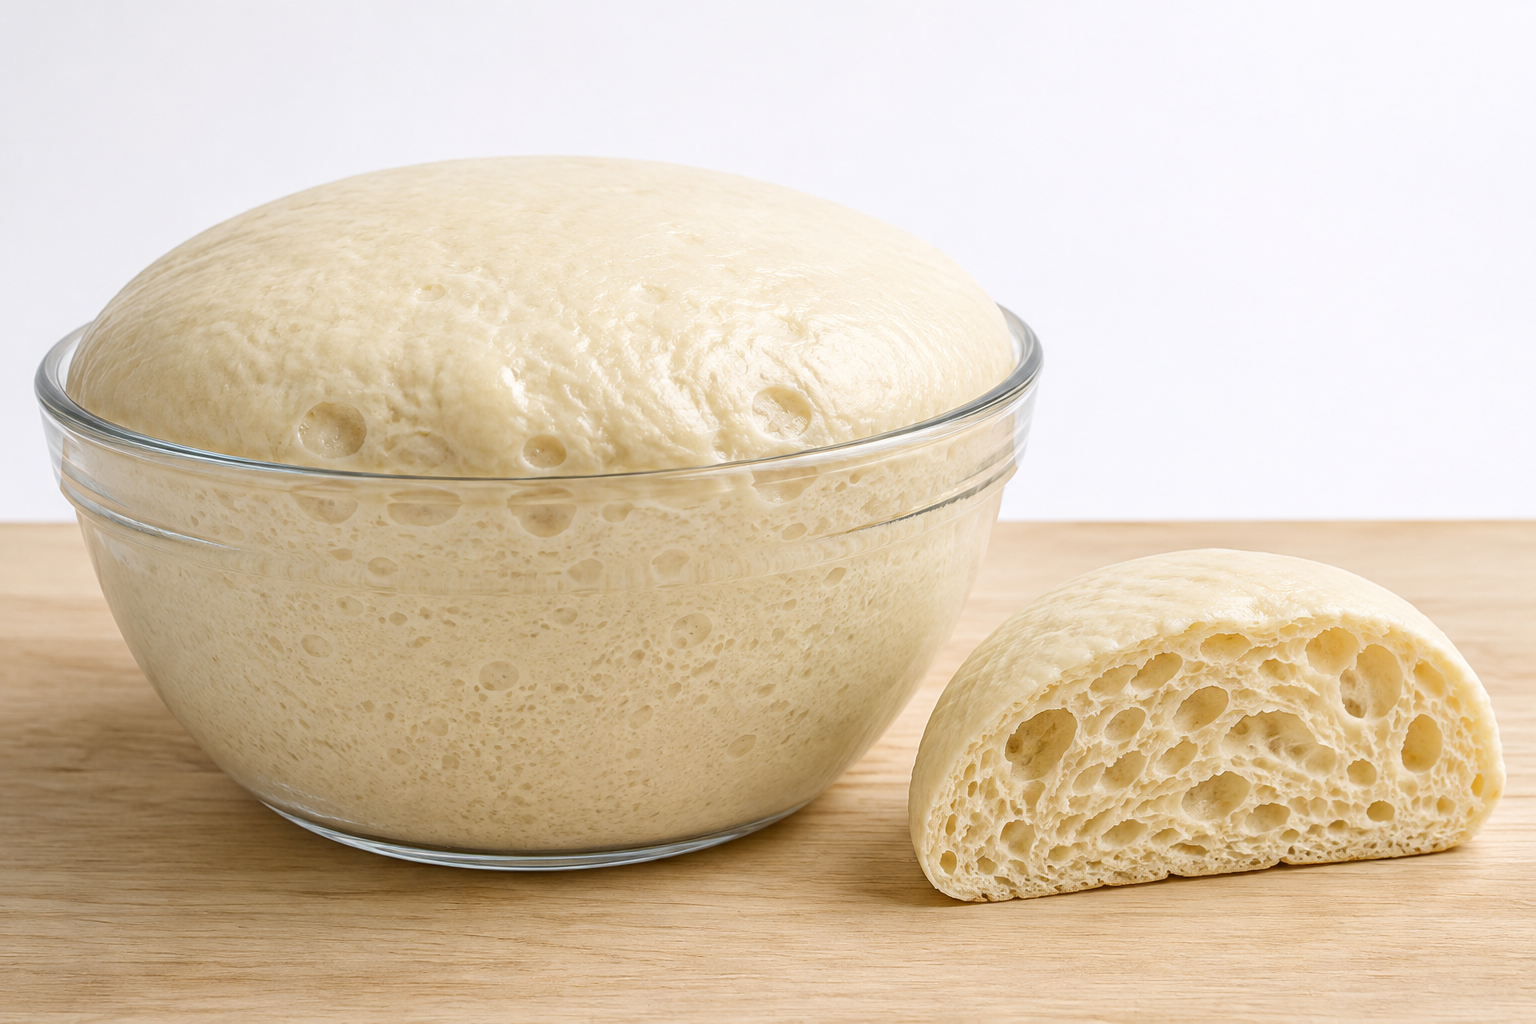
\includegraphics[width=0.96\linewidth]{images/book3/ai/b3-15-bread-dough-risen.png}
\end{minipage}

{\small A la izquierda: levadura de panadería, gemando. A la derecha: lo que
su \omterm{def:b1:respiration-fermentation:fermentation}{fermentación} le hace a la masa: el $\mathrm{CO_2}$ del equivalente a dos
\omterm{def:b1:water-small-molecules:atp}{ATP} de \omterm{def:b1:respiration-fermentation:glycolysis}{glucólisis} por glucosa, atrapado en el gluten. El etanol se evapora
al hornear.}
\end{omfigure}

\begin{proposition}[El efecto Pasteur]\label{prop:b1:respiration-fermentation:pasteur}
\index{efecto Pasteur}
Una \omterm{def:b1:cell-unit-of-life:cell}{célula} capaz de respirar consume glucosa mucho más deprisa cuando se le
priva de oxígeno que cuando se le suministra, y crece mucho menos con ella.
\end{proposition}
\begin{proof}[Evidencia]
Pasteur (1861) encontró que la levadura de una cuba aireada consumía azúcar
despacio y se multiplicaba, mientras que en una cuba cerrada lo consumía
diez veces más deprisa, se multiplicaba poco y fabricaba alcohol. La
explicación es el rendimiento en \omterm{def:b1:water-small-molecules:atp}{ATP}: para obtener el mismo \omterm{def:b1:water-small-molecules:atp}{ATP} a 2 por
glucosa que a 30, la \omterm{def:b1:cell-unit-of-life:cell}{célula} debe hacer funcionar la \omterm{def:b1:respiration-fermentation:glycolysis}{glucólisis} quince veces
más deprisa, y la PFK, liberada de la inhibición por \omterm{def:b1:water-small-molecules:atp}{ATP} y citrato que
mantiene la respiración, se lo permite. Un músculo que esprinta muestra el
mismo efecto en cuestión de segundos: su \omterm{def:b1:carbohydrates:polysaccharide}{glucógeno} cae veinte veces más
deprisa que en reposo y el lactato sube.
\end{proof}

\begin{definition}[Cociente respiratorio]\label{def:b1:respiration-fermentation:rq}
\index{cociente respiratorio}
El \emph{cociente respiratorio} CR es la razón entre el $\mathrm{CO_2}$
producido y el $\mathrm{O_2}$ consumido, en moles. Los \omterm{def:b1:carbohydrates:monosaccharide}{glúcidos} dan 1,0
(seis de cada uno por glucosa); las \omterm{def:b1:lipids:triglyceride}{grasas}, unos 0,7 (palmitato:
$\mathrm{C_{16}H_{32}O_2} + 23\,\mathrm{O_2} \to 16\,\mathrm{CO_2} +
16\,\mathrm{H_2O}$, $16/23 = 0.70$), porque sus carbonos están más reducidos
y necesitan más oxígeno por $\mathrm{CO_2}$; las \omterm{def:b1:proteins:peptide}{proteínas}, unos 0,8. Un
cultivo que fermenta libera $\mathrm{CO_2}$ sin tomar oxígeno: su CR es
infinito, y un CR superior a 1 en un cultivo mixto mide la proporción de
\omterm{def:b1:respiration-fermentation:fermentation}{fermentación}. Medido en un animal entero por análisis de gases, el CR indica
qué combustible está quemando.
\end{definition}

\begin{example}[Leer un cociente respiratorio]\label{ex:b1:respiration-fermentation:readrq}
Un ser humano en reposo tras una comida rica en \omterm{def:b1:carbohydrates:monosaccharide}{glúcidos}: CR 0,95, quema
glucosa. La misma persona tras una noche de ayuno: 0,75, \omterm{def:b1:lipids:triglyceride}{grasa}. Un
maratoniano en el kilómetro treinta, con el \omterm{def:b1:carbohydrates:polysaccharide}{glucógeno} agotado: 0,72. Un
matraz de levadura con glucosa y un poco de aire: CR 4; tres cuartas partes
de su glucosa se están fermentando.
\end{example}

\section{Otros combustibles y la regulación del conjunto}

\begin{proposition}[Las grasas y las proteínas entran en la misma maquinaria]\label{prop:b1:respiration-fermentation:otherfuels}
\index{beta-oxidation@$\beta$-oxidación}
Los \omterm{def:b1:lipids:fattyacid}{ácidos grasos} se activan a acil-CoA y, en la \omterm{def:b1:eukaryotic-cell:mitochondrion}{matriz mitocondrial}, se
acortan de dos en dos carbonos por la \emph{$\beta$-oxidación}, y cada
vuelta rinde un \omterm{def:b1:respiration-fermentation:pdh}{acetil-CoA}, un NADH y un $\mathrm{FADH_2}$: el palmitato
(C16) da 8 \omterm{def:b1:respiration-fermentation:pdh}{acetil-CoA}, 7 NADH y 7 $\mathrm{FADH_2}$, unos 106 \omterm{def:b1:water-small-molecules:atp}{ATP}, o
\qty{6.6}{} \omterm{def:b1:water-small-molecules:atp}{ATP} por carbono frente a los 5 de la glucosa. Los \omterm{def:b1:proteins:aminoacid}{aminoácidos}
pierden su nitrógeno como amoniaco (convertido en urea en el hígado) y sus
esqueletos carbonados entran como piruvato, \omterm{def:b1:respiration-fermentation:pdh}{acetil-CoA} o intermediarios del
\omterm{def:b1:respiration-fermentation:krebs}{ciclo de Krebs}. Todos los combustibles convergen en el \omterm{def:b1:respiration-fermentation:pdh}{acetil-CoA} y en la
cadena; la \omterm{def:b1:cell-unit-of-life:cell}{célula} elige entre ellos según las hormonas y según el estado de
su \omterm{def:b1:water-small-molecules:atp}{ATP}, como describe el \cref{ch:b1:biosyntheses-integration}.
\end{proposition}

\begin{example}[Un gramo de cada]\label{ex:b1:respiration-fermentation:gramofeach}
Un gramo de glucosa (\qty{5.6}{mmol}) rinde unos \qty{170}{mmol} de \omterm{def:b1:water-small-molecules:atp}{ATP}; un
gramo de palmitato (\qty{3.9}{mmol}), unos \qty{410}{mmol}: los
\qty{38}{kJ/g} frente a los \qty{17}{kJ/g} del \cref{ch:b1:lipids},
convertidos en moneda. La \omterm{def:b1:lipids:triglyceride}{grasa} cuesta más oxígeno por \omterm{def:b1:water-small-molecules:atp}{ATP}, y por eso el
músculo de un velocista, limitado por el oxígeno, quema \omterm{def:b1:carbohydrates:polysaccharide}{glucógeno}, y un ave
migradora, con oxígeno de sobra y limitada por la masa, quema \omterm{def:b1:lipids:triglyceride}{grasa}.
\end{example}

\section{Ejercicios}

\begin{exercise}[$\star$]\label{exo:b1:respiration-fermentation:1}
Nómbrense las tres etapas de la respiración, su localización y lo que
produce cada una.
\end{exercise}

\begin{exercise}[$\star$]\label{exo:b1:respiration-fermentation:2}
Escríbase el balance de la \omterm{def:b1:respiration-fermentation:glycolysis}{glucólisis} y explíquese qué es la
``\omterm{def:b1:respiration-fermentation:glycolysis}{fosforilación a nivel de sustrato}''.
\end{exercise}

\begin{exercise}[$\star$]\label{exo:b1:respiration-fermentation:3}
A partir de la figura del \omterm{def:b1:respiration-fermentation:krebs}{ciclo de Krebs}, enumérense por orden los productos
liberados en una vuelta, y dígase de dónde proceden los dos
$\mathrm{CO_2}$.
\end{exercise}

\begin{exercise}[$\star$]\label{exo:b1:respiration-fermentation:4}
¿Qué consigue la \omterm{def:b1:respiration-fermentation:fermentation}{fermentación} para una \omterm{def:b1:cell-unit-of-life:cell}{célula} sin oxígeno, y qué no
consigue?
\end{exercise}

\begin{exercise}[$\star\star$]\label{exo:b1:respiration-fermentation:5}
Calcúlese $\Delta G^{\circ\prime}$ para la transferencia de dos electrones
desde el NADH ($E'_0 = \qty{-0.32}{V}$) al oxígeno (\qty{+0.82}{V}), y a la
ubiquinona (\qty{+0.05}{V}). ¿Cuántos \omterm{def:b1:water-small-molecules:atp}{ATP} podría pagar cada paso en
principio?
\end{exercise}

\begin{exercise}[$\star\star$]\label{exo:b1:respiration-fermentation:6}
Establézcase el balance de \omterm{def:b1:water-small-molecules:atp}{ATP} de una glucosa en una \omterm{def:b1:cell-unit-of-life:cell}{célula} muscular
(lanzadera del glicerol fosfato) y en una \omterm{def:b1:cell-unit-of-life:cell}{célula} hepática (lanzadera del
malato), con relaciones P/O de 2,5 y 1,5.
\end{exercise}

\begin{exercise}[$\star\star$]\label{exo:b1:respiration-fermentation:7}
Un cultivo consume \qty{1.0}{mmol} de $\mathrm{O_2}$ y libera
\qty{2.2}{mmol} de $\mathrm{CO_2}$ por hora con glucosa. Calcúlense el CR y
las fracciones de glucosa respirada y fermentada.
\end{exercise}

\begin{exercise}[$\star\star$]\label{exo:b1:respiration-fermentation:8}
Explíquese qué les ocurre al consumo de oxígeno, a la síntesis de \omterm{def:b1:water-small-molecules:atp}{ATP} y a la
producción de calor cuando se añade dinitrofenol a \omterm{def:b1:eukaryotic-cell:mitochondrion}{mitocondrias} que respiran,
y por qué el fármaco era letal.
\end{exercise}

\begin{exercise}[$\star\star$]\label{exo:b1:respiration-fermentation:9}
El cianuro bloquea el complejo IV. Predíganse su efecto sobre la \omterm{def:b1:respiration-fermentation:chain}{cadena
respiratoria}, sobre el \omterm{def:b1:respiration-fermentation:krebs}{ciclo de Krebs} y sobre la \omterm{def:b1:respiration-fermentation:glycolysis}{glucólisis} de una \omterm{def:b1:cell-unit-of-life:cell}{célula}, y
explíquese por qué se acumula lactato en la sangre de los envenenados.
\end{exercise}

\begin{exercise}[$\star\star\star$]\label{exo:b1:respiration-fermentation:10}
Calcúlense el rendimiento en \omterm{def:b1:water-small-molecules:atp}{ATP} del palmitato (8 \omterm{def:b1:respiration-fermentation:pdh}{acetil-CoA}, 7 NADH, 7
$\mathrm{FADH_2}$, menos 2 \omterm{def:b1:water-small-molecules:atp}{ATP} de la activación) y su rendimiento por
carbono; calcúlese el oxígeno consumido por \omterm{def:b1:water-small-molecules:atp}{ATP} para el palmitato y para la
glucosa. ¿Qué combustible debería preferir una foca que bucea, y cuál un
colibrí?
\end{exercise}

\begin{exercise}[$\star\star\star$]\label{exo:b1:respiration-fermentation:11}
Una fibra muscular contiene \qty{5}{mmol/L} de \omterm{def:b1:water-small-molecules:atp}{ATP} y consume
\qty{3}{mmol/L} por segundo en un esprint. ¿Cuánto duraría su \omterm{def:b1:water-small-molecules:atp}{ATP} por sí
solo? Su fosfocreatina (\qty{25}{mmol/L}) regenera \omterm{def:b1:water-small-molecules:atp}{ATP} uno a uno; su
\omterm{def:b1:carbohydrates:polysaccharide}{glucógeno}, mediante \omterm{def:b1:respiration-fermentation:fermentation}{fermentación}, da 3 \omterm{def:b1:water-small-molecules:atp}{ATP} por unidad de glucosa hasta un
máximo de \qty{2}{mmol/L} de unidades de glucosa por segundo. Calcúlese el
tiempo que cada reserva puede sostener el esprint, y explíquese por qué una
carrera de 100 m se corre casi por completo sin oxígeno.
\end{exercise}

\begin{exercise}[$\star\star\star$]\label{exo:b1:respiration-fermentation:12}
``La \omterm{def:b1:eukaryotic-cell:mitochondrion}{mitocondria} es una batería que los electrones cargan y que se descarga
a través de una turbina.'' Discútase en un párrafo: qué almacena el
gradiente, qué hace la sintasa, y dónde la analogía es exacta y dónde es
vaga.
\end{exercise}

\section{Problema: levadura con aire y sin aire}

\begin{problem}[{Problema de fin de semana --- las cubas de Pasteur
revisitadas: ATP contado, glucosa consumida, biomasa crecida y gases
medidos, hasta llegar al cociente de rendimientos en ATP y a la relación
P/O}]
\label{pb:b1:respiration-fermentation:1}
Se cultiva levadura con glucosa en dos matraces idénticos, uno aireado y
otro cerrado. Úsense relaciones P/O de 2,5 (NADH) y 1,5
($\mathrm{FADH_2}$), la lanzadera de $\mathrm{FADH_2}$ para el NADH
citosólico, un rendimiento de crecimiento de \qty{10.5}{g} de biomasa seca
por mol de \omterm{def:b1:water-small-molecules:atp}{ATP} y glucosa a \qty{180}{g/mol}.

\medskip
\noindent\textbf{Parte I --- \omterm{def:b1:water-small-molecules:atp}{ATP} contado.}
\begin{enumerate}
  \item Enumérense el \omterm{def:b1:water-small-molecules:atp}{ATP}, el GTP, el NADH y el $\mathrm{FADH_2}$
        producidos a partir de una glucosa por la \omterm{def:b1:respiration-fermentation:glycolysis}{glucólisis}, la piruvato
        deshidrogenasa y el \omterm{def:b1:respiration-fermentation:krebs}{ciclo de Krebs}.
  \item Calcúlense los protones bombeados por la cadena por glucosa (10 por
        cada NADH mitocondrial, 6 por $\mathrm{FADH_2}$; el NADH citosólico
        entra como $\mathrm{FADH_2}$).
  \item Calcúlense el \omterm{def:b1:water-small-molecules:atp}{ATP} fabricado por la sintasa a \qty{4}{H^+} por \omterm{def:b1:water-small-molecules:atp}{ATP} y
        el \omterm{def:b1:water-small-molecules:atp}{ATP} total por glucosa con aire.
  \item Calcúlese el \omterm{def:b1:water-small-molecules:atp}{ATP} por glucosa sin aire.
  \item Calcúlese el cociente entre los dos rendimientos.
  \item Calcúlese la \omterm{prop:b1:water-small-molecules:gibbs}{energía libre} capturada con aire
        ($\Delta G_{\text{ATP}}
        = \qty{-50}{kJ/mol}$) como fracción de los
        \qty{2870}{kJ}, y sin aire como fracción de esos \qty{2870}{kJ} y
        de la energía realmente liberada por la \omterm{def:b1:respiration-fermentation:fermentation}{fermentación} (glucosa a dos
        etanoles y dos $\mathrm{CO_2}$: \qty{-235}{kJ/mol}).
\end{enumerate}

\medskip
\noindent\textbf{Parte II --- Glucosa consumida, biomasa crecida.}
El matraz cerrado debe fabricar \omterm{def:b1:water-small-molecules:atp}{ATP} a la misma velocidad que el aireado para
mantener sus \omterm{def:b1:cell-unit-of-life:cell}{células}: \qty{30}{mmol} de \omterm{def:b1:water-small-molecules:atp}{ATP} por hora.
\begin{enumerate}[resume]
  \item Calcúlese la glucosa consumida por hora en cada matraz.
  \item Calcúlense el etanol y el $\mathrm{CO_2}$ producidos por hora en el
        matraz cerrado, y el $\mathrm{CO_2}$ y el $\mathrm{O_2}$
        intercambiados en el aireado.
  \item Calcúlese la biomasa que el matraz cerrado puede construir por mol
        de glucosa y por gramo de glucosa.
  \item El matraz aireado construye \qty{0.5}{g} de biomasa por gramo de
        glucosa. Calcúlese el \omterm{def:b1:water-small-molecules:atp}{ATP} que eso representaría a \qty{10.5}{g/mol},
        y compárese con los 30 \omterm{def:b1:water-small-molecules:atp}{ATP} disponibles. ¿Qué limita el rendimiento
        aerobio?
  \item Explíquese el \omterm{prop:b1:respiration-fermentation:pasteur}{efecto Pasteur} a partir de las preguntas 7 y 9, y
        nómbrese la \omterm{def:b1:enzymes:enzyme}{enzima} cuya regulación lo lleva a cabo.
\end{enumerate}

\medskip
\noindent\textbf{Parte III --- Gases medidos.}
Un tercer matraz, mal aireado, libera \qty{44}{mg} de $\mathrm{CO_2}$ y
consume \qty{20}{mg} de $\mathrm{O_2}$ por hora.
\begin{enumerate}[resume]
  \item Conviértanse ambos a milimoles y calcúlese el CR.
  \item Sea $x$ la glucosa respirada e $y$ la glucosa fermentada por hora.
        Escríbanse los balances de $\mathrm{O_2}$ y de $\mathrm{CO_2}$ y
        despéjense $x$ e $y$.
  \item ¿Qué fracción de la glucosa se fermenta? ¿Qué fracción del \omterm{def:b1:water-small-molecules:atp}{ATP}
        procede de la \omterm{def:b1:respiration-fermentation:fermentation}{fermentación}?
  \item Ese mismo matraz con palmitato en vez de glucosa (en aerobiosis):
        calcúlese el CR.
  \item Un estudiante mide un CR de 0,7 en un animal en reposo tras una
        noche de ayuno y de 1,0 tras una comida. Interprétese.
\end{enumerate}

\medskip
\noindent\textbf{Parte IV --- La turbina.}
\begin{enumerate}[resume]
  \item Calcúlese la \omterm{prop:b1:water-small-molecules:gibbs}{energía libre} de un mol de protones que atraviesan una
        \omterm{thm:b1:respiration-fermentation:chemiosmosis}{fuerza protón-motriz} de \qty{0.22}{V}.
  \item Calcúlense la energía de \qty{4}{H^+} y el rendimiento de la
        sintasa a \qty{50}{kJ} por \omterm{def:b1:water-small-molecules:atp}{ATP}.
  \item Calcúlense la \omterm{prop:b1:water-small-molecules:gibbs}{energía libre} liberada por dos electrones que caen
        del NADH al $\mathrm{O_2}$ (\qty{1.14}{V}), la energía almacenada
        en los diez protones bombeados y el rendimiento de la cadena.
  \item Combínense los dos rendimientos y compárese con 2,5 \omterm{def:b1:water-small-molecules:atp}{ATP} $\times$
        \qty{50}{kJ} sobre \qty{220}{kJ}.
  \item Se añade un desacoplante al matraz aireado. Predíganse los cambios
        en el consumo de oxígeno, el rendimiento en \omterm{def:b1:water-small-molecules:atp}{ATP}, el consumo de
        glucosa, la producción de calor y el crecimiento.
  \item Se añade en su lugar oligomicina, que bloquea la sintasa.
        Predíganse los cambios, y qué ocurre si después se añade encima un
        desacoplante.
  \item Una levadura mutante carece del complejo I; su NADH entra en la
        cadena por una \omterm{def:b1:enzymes:enzyme}{enzima} alternativa que no bombea protones.
        Calcúlense su \omterm{thm:b1:respiration-fermentation:chemiosmosis}{relación P/O} para el NADH y su \omterm{def:b1:water-small-molecules:atp}{ATP} por glucosa.
  \item Explíquese por qué la \omterm{def:b1:cell-unit-of-life:cell}{célula} mantiene la reserva de NADH
        mitocondrial casi totalmente reducida cuando falta el oxígeno, y
        qué le hace eso al \omterm{def:b1:respiration-fermentation:krebs}{ciclo de Krebs}.
  \item Enúnciese el resultado: el \omterm{def:b1:water-small-molecules:atp}{ATP} por glucosa con aire y sin aire, su
        cociente, y las relaciones P/O del NADH y del $\mathrm{FADH_2}$.
\end{enumerate}
\end{problem}
